% Created by tikzDevice version 0.12.6 on 2024-11-19 16:55:52
% !TEX encoding = UTF-8 Unicode
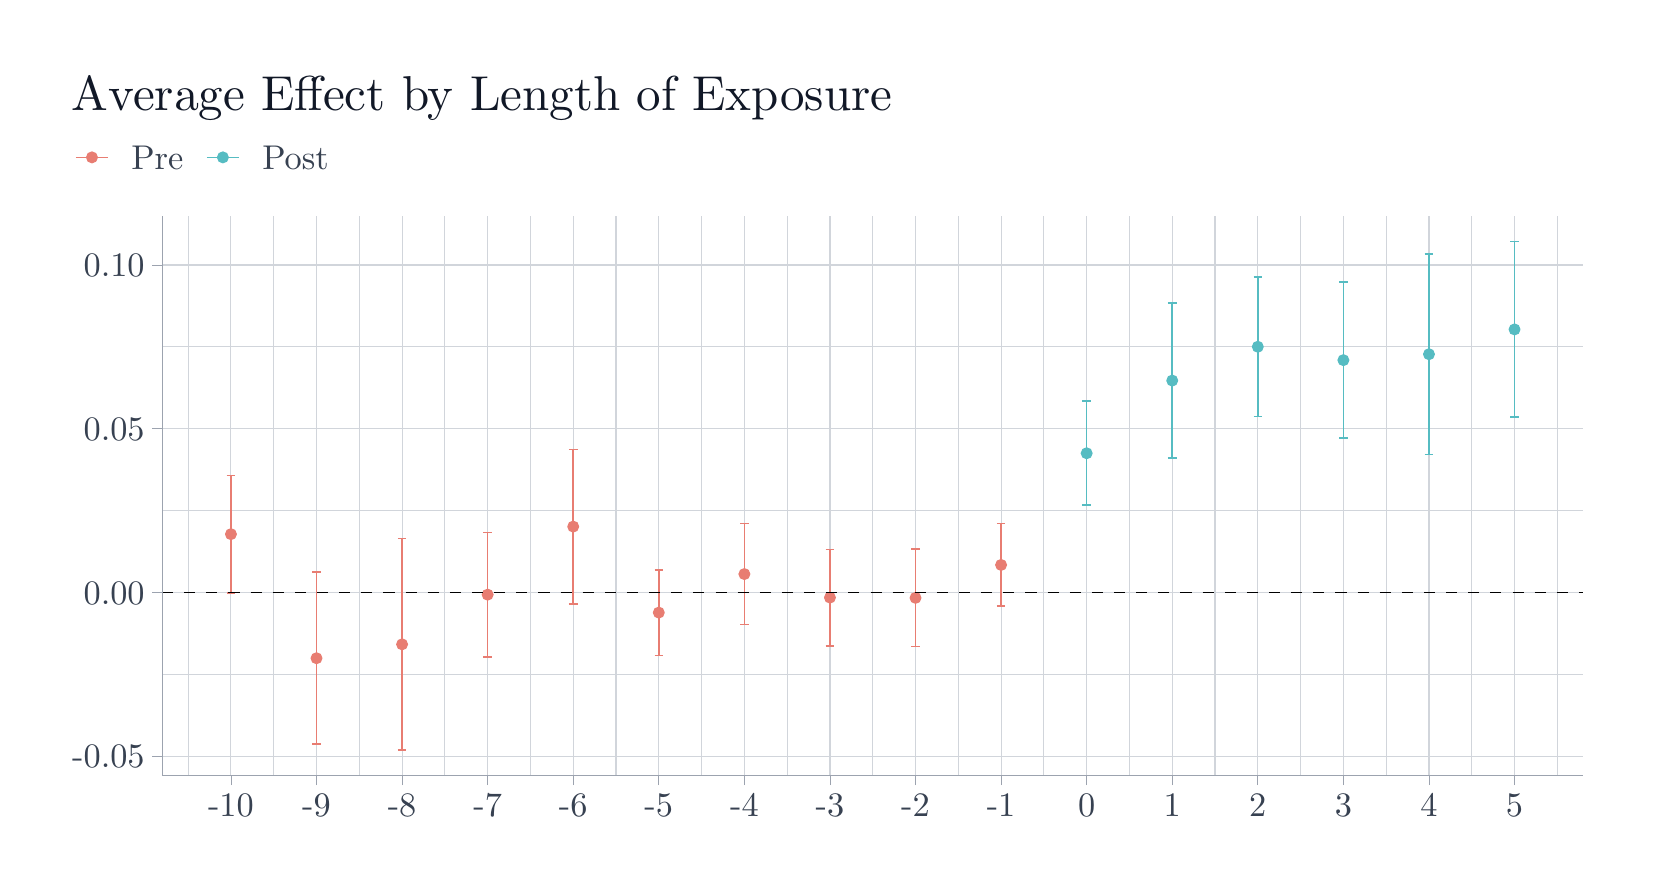
\begin{tikzpicture}[x=1pt,y=1pt]
\definecolor{fillColor}{RGB}{255,255,255}
\path[use as bounding box,fill=fillColor] (0,0) rectangle (578.16,303.53);
\begin{scope}
\path[clip] (  0.00,  0.00) rectangle (578.16,303.53);
\definecolor{drawColor}{RGB}{255,255,255}

\path[draw=drawColor,line width= 0.7pt,line join=round,line cap=round,fill=fillColor] (  0.00,  0.00) rectangle (578.16,303.53);
\end{scope}
\begin{scope}
\path[clip] ( 48.56, 33.29) rectangle (562.16,235.43);
\definecolor{drawColor}{RGB}{255,255,255}
\definecolor{fillColor}{RGB}{255,255,255}

\path[draw=drawColor,line width= 0.7pt,line join=round,line cap=round,fill=fillColor] ( 48.56, 33.29) rectangle (562.16,235.43);
\definecolor{drawColor}{RGB}{209,213,219}

\path[draw=drawColor,line width= 0.4pt,line join=round] ( 48.56, 69.89) --
	(562.16, 69.89);

\path[draw=drawColor,line width= 0.4pt,line join=round] ( 48.56,129.04) --
	(562.16,129.04);

\path[draw=drawColor,line width= 0.4pt,line join=round] ( 48.56,188.19) --
	(562.16,188.19);

\path[draw=drawColor,line width= 0.4pt,line join=round] ( 57.99, 33.29) --
	( 57.99,235.43);

\path[draw=drawColor,line width= 0.4pt,line join=round] ( 88.91, 33.29) --
	( 88.91,235.43);

\path[draw=drawColor,line width= 0.4pt,line join=round] (119.83, 33.29) --
	(119.83,235.43);

\path[draw=drawColor,line width= 0.4pt,line join=round] (150.75, 33.29) --
	(150.75,235.43);

\path[draw=drawColor,line width= 0.4pt,line join=round] (181.67, 33.29) --
	(181.67,235.43);

\path[draw=drawColor,line width= 0.4pt,line join=round] (212.59, 33.29) --
	(212.59,235.43);

\path[draw=drawColor,line width= 0.4pt,line join=round] (243.52, 33.29) --
	(243.52,235.43);

\path[draw=drawColor,line width= 0.4pt,line join=round] (274.44, 33.29) --
	(274.44,235.43);

\path[draw=drawColor,line width= 0.4pt,line join=round] (305.36, 33.29) --
	(305.36,235.43);

\path[draw=drawColor,line width= 0.4pt,line join=round] (336.28, 33.29) --
	(336.28,235.43);

\path[draw=drawColor,line width= 0.4pt,line join=round] (367.20, 33.29) --
	(367.20,235.43);

\path[draw=drawColor,line width= 0.4pt,line join=round] (398.12, 33.29) --
	(398.12,235.43);

\path[draw=drawColor,line width= 0.4pt,line join=round] (429.04, 33.29) --
	(429.04,235.43);

\path[draw=drawColor,line width= 0.4pt,line join=round] (459.96, 33.29) --
	(459.96,235.43);

\path[draw=drawColor,line width= 0.4pt,line join=round] (490.89, 33.29) --
	(490.89,235.43);

\path[draw=drawColor,line width= 0.4pt,line join=round] (521.81, 33.29) --
	(521.81,235.43);

\path[draw=drawColor,line width= 0.4pt,line join=round] (552.73, 33.29) --
	(552.73,235.43);

\path[draw=drawColor,line width= 0.4pt,line join=round] ( 48.56, 40.32) --
	(562.16, 40.32);

\path[draw=drawColor,line width= 0.4pt,line join=round] ( 48.56, 99.47) --
	(562.16, 99.47);

\path[draw=drawColor,line width= 0.4pt,line join=round] ( 48.56,158.62) --
	(562.16,158.62);

\path[draw=drawColor,line width= 0.4pt,line join=round] ( 48.56,217.77) --
	(562.16,217.77);

\path[draw=drawColor,line width= 0.4pt,line join=round] ( 73.45, 33.29) --
	( 73.45,235.43);

\path[draw=drawColor,line width= 0.4pt,line join=round] (104.37, 33.29) --
	(104.37,235.43);

\path[draw=drawColor,line width= 0.4pt,line join=round] (135.29, 33.29) --
	(135.29,235.43);

\path[draw=drawColor,line width= 0.4pt,line join=round] (166.21, 33.29) --
	(166.21,235.43);

\path[draw=drawColor,line width= 0.4pt,line join=round] (197.13, 33.29) --
	(197.13,235.43);

\path[draw=drawColor,line width= 0.4pt,line join=round] (228.05, 33.29) --
	(228.05,235.43);

\path[draw=drawColor,line width= 0.4pt,line join=round] (258.98, 33.29) --
	(258.98,235.43);

\path[draw=drawColor,line width= 0.4pt,line join=round] (289.90, 33.29) --
	(289.90,235.43);

\path[draw=drawColor,line width= 0.4pt,line join=round] (320.82, 33.29) --
	(320.82,235.43);

\path[draw=drawColor,line width= 0.4pt,line join=round] (351.74, 33.29) --
	(351.74,235.43);

\path[draw=drawColor,line width= 0.4pt,line join=round] (382.66, 33.29) --
	(382.66,235.43);

\path[draw=drawColor,line width= 0.4pt,line join=round] (413.58, 33.29) --
	(413.58,235.43);

\path[draw=drawColor,line width= 0.4pt,line join=round] (444.50, 33.29) --
	(444.50,235.43);

\path[draw=drawColor,line width= 0.4pt,line join=round] (475.43, 33.29) --
	(475.43,235.43);

\path[draw=drawColor,line width= 0.4pt,line join=round] (506.35, 33.29) --
	(506.35,235.43);

\path[draw=drawColor,line width= 0.4pt,line join=round] (537.27, 33.29) --
	(537.27,235.43);
\definecolor{drawColor}{RGB}{232,125,114}
\definecolor{fillColor}{RGB}{232,125,114}

\path[draw=drawColor,line width= 0.4pt,line join=round,line cap=round,fill=fillColor] ( 73.45,120.51) circle (  1.96);

\path[draw=drawColor,line width= 0.4pt,line join=round,line cap=round,fill=fillColor] (104.37, 75.68) circle (  1.96);

\path[draw=drawColor,line width= 0.4pt,line join=round,line cap=round,fill=fillColor] (135.29, 80.70) circle (  1.96);

\path[draw=drawColor,line width= 0.4pt,line join=round,line cap=round,fill=fillColor] (166.21, 98.65) circle (  1.96);

\path[draw=drawColor,line width= 0.4pt,line join=round,line cap=round,fill=fillColor] (197.13,123.24) circle (  1.96);

\path[draw=drawColor,line width= 0.4pt,line join=round,line cap=round,fill=fillColor] (228.05, 92.17) circle (  1.96);

\path[draw=drawColor,line width= 0.4pt,line join=round,line cap=round,fill=fillColor] (258.98,106.09) circle (  1.96);

\path[draw=drawColor,line width= 0.4pt,line join=round,line cap=round,fill=fillColor] (289.90, 97.59) circle (  1.96);

\path[draw=drawColor,line width= 0.4pt,line join=round,line cap=round,fill=fillColor] (320.82, 97.49) circle (  1.96);

\path[draw=drawColor,line width= 0.4pt,line join=round,line cap=round,fill=fillColor] (351.74,109.39) circle (  1.96);
\definecolor{drawColor}{RGB}{86,188,194}
\definecolor{fillColor}{RGB}{86,188,194}

\path[draw=drawColor,line width= 0.4pt,line join=round,line cap=round,fill=fillColor] (382.66,149.74) circle (  1.96);

\path[draw=drawColor,line width= 0.4pt,line join=round,line cap=round,fill=fillColor] (413.58,176.01) circle (  1.96);

\path[draw=drawColor,line width= 0.4pt,line join=round,line cap=round,fill=fillColor] (444.50,188.23) circle (  1.96);

\path[draw=drawColor,line width= 0.4pt,line join=round,line cap=round,fill=fillColor] (475.43,183.39) circle (  1.96);

\path[draw=drawColor,line width= 0.4pt,line join=round,line cap=round,fill=fillColor] (506.35,185.53) circle (  1.96);

\path[draw=drawColor,line width= 0.4pt,line join=round,line cap=round,fill=fillColor] (537.27,194.49) circle (  1.96);
\definecolor{drawColor}{RGB}{232,125,114}

\path[draw=drawColor,line width= 0.6pt,line join=round] ( 71.90,141.70) --
	( 74.99,141.70);

\path[draw=drawColor,line width= 0.6pt,line join=round] ( 73.45,141.70) --
	( 73.45, 99.31);

\path[draw=drawColor,line width= 0.6pt,line join=round] ( 71.90, 99.31) --
	( 74.99, 99.31);

\path[draw=drawColor,line width= 0.6pt,line join=round] (102.82,106.76) --
	(105.92,106.76);

\path[draw=drawColor,line width= 0.6pt,line join=round] (104.37,106.76) --
	(104.37, 44.59);

\path[draw=drawColor,line width= 0.6pt,line join=round] (102.82, 44.59) --
	(105.92, 44.59);

\path[draw=drawColor,line width= 0.6pt,line join=round] (133.74,118.94) --
	(136.84,118.94);

\path[draw=drawColor,line width= 0.6pt,line join=round] (135.29,118.94) --
	(135.29, 42.47);

\path[draw=drawColor,line width= 0.6pt,line join=round] (133.74, 42.47) --
	(136.84, 42.47);

\path[draw=drawColor,line width= 0.6pt,line join=round] (164.67,121.08) --
	(167.76,121.08);

\path[draw=drawColor,line width= 0.6pt,line join=round] (166.21,121.08) --
	(166.21, 76.22);

\path[draw=drawColor,line width= 0.6pt,line join=round] (164.67, 76.22) --
	(167.76, 76.22);

\path[draw=drawColor,line width= 0.6pt,line join=round] (195.59,151.11) --
	(198.68,151.11);

\path[draw=drawColor,line width= 0.6pt,line join=round] (197.13,151.11) --
	(197.13, 95.38);

\path[draw=drawColor,line width= 0.6pt,line join=round] (195.59, 95.38) --
	(198.68, 95.38);

\path[draw=drawColor,line width= 0.6pt,line join=round] (226.51,107.66) --
	(229.60,107.66);

\path[draw=drawColor,line width= 0.6pt,line join=round] (228.05,107.66) --
	(228.05, 76.69);

\path[draw=drawColor,line width= 0.6pt,line join=round] (226.51, 76.69) --
	(229.60, 76.69);

\path[draw=drawColor,line width= 0.6pt,line join=round] (257.43,124.33) --
	(260.52,124.33);

\path[draw=drawColor,line width= 0.6pt,line join=round] (258.98,124.33) --
	(258.98, 87.85);

\path[draw=drawColor,line width= 0.6pt,line join=round] (257.43, 87.85) --
	(260.52, 87.85);

\path[draw=drawColor,line width= 0.6pt,line join=round] (288.35,115.02) --
	(291.44,115.02);

\path[draw=drawColor,line width= 0.6pt,line join=round] (289.90,115.02) --
	(289.90, 80.16);

\path[draw=drawColor,line width= 0.6pt,line join=round] (288.35, 80.16) --
	(291.44, 80.16);

\path[draw=drawColor,line width= 0.6pt,line join=round] (319.27,115.08) --
	(322.36,115.08);

\path[draw=drawColor,line width= 0.6pt,line join=round] (320.82,115.08) --
	(320.82, 79.90);

\path[draw=drawColor,line width= 0.6pt,line join=round] (319.27, 79.90) --
	(322.36, 79.90);

\path[draw=drawColor,line width= 0.6pt,line join=round] (350.19,124.32) --
	(353.29,124.32);

\path[draw=drawColor,line width= 0.6pt,line join=round] (351.74,124.32) --
	(351.74, 94.45);

\path[draw=drawColor,line width= 0.6pt,line join=round] (350.19, 94.45) --
	(353.29, 94.45);
\definecolor{drawColor}{RGB}{86,188,194}

\path[draw=drawColor,line width= 0.6pt,line join=round] (381.12,168.53) --
	(384.21,168.53);

\path[draw=drawColor,line width= 0.6pt,line join=round] (382.66,168.53) --
	(382.66,130.94);

\path[draw=drawColor,line width= 0.6pt,line join=round] (381.12,130.94) --
	(384.21,130.94);

\path[draw=drawColor,line width= 0.6pt,line join=round] (412.04,204.03) --
	(415.13,204.03);

\path[draw=drawColor,line width= 0.6pt,line join=round] (413.58,204.03) --
	(413.58,147.99);

\path[draw=drawColor,line width= 0.6pt,line join=round] (412.04,147.99) --
	(415.13,147.99);

\path[draw=drawColor,line width= 0.6pt,line join=round] (442.96,213.47) --
	(446.05,213.47);

\path[draw=drawColor,line width= 0.6pt,line join=round] (444.50,213.47) --
	(444.50,162.98);

\path[draw=drawColor,line width= 0.6pt,line join=round] (442.96,162.98) --
	(446.05,162.98);

\path[draw=drawColor,line width= 0.6pt,line join=round] (473.88,211.56) --
	(476.97,211.56);

\path[draw=drawColor,line width= 0.6pt,line join=round] (475.43,211.56) --
	(475.43,155.22);

\path[draw=drawColor,line width= 0.6pt,line join=round] (473.88,155.22) --
	(476.97,155.22);

\path[draw=drawColor,line width= 0.6pt,line join=round] (504.80,221.73) --
	(507.89,221.73);

\path[draw=drawColor,line width= 0.6pt,line join=round] (506.35,221.73) --
	(506.35,149.33);

\path[draw=drawColor,line width= 0.6pt,line join=round] (504.80,149.33) --
	(507.89,149.33);

\path[draw=drawColor,line width= 0.6pt,line join=round] (535.72,226.24) --
	(538.81,226.24);

\path[draw=drawColor,line width= 0.6pt,line join=round] (537.27,226.24) --
	(537.27,162.73);

\path[draw=drawColor,line width= 0.6pt,line join=round] (535.72,162.73) --
	(538.81,162.73);
\definecolor{drawColor}{RGB}{0,0,0}

\path[draw=drawColor,line width= 0.6pt,dash pattern=on 4pt off 4pt ,line join=round] ( 48.56, 99.47) -- (562.16, 99.47);
\end{scope}
\begin{scope}
\path[clip] (  0.00,  0.00) rectangle (578.16,303.53);
\definecolor{drawColor}{RGB}{156,163,175}

\path[draw=drawColor,line width= 0.3pt,line join=round] ( 48.56, 33.29) --
	( 48.56,235.43);
\end{scope}
\begin{scope}
\path[clip] (  0.00,  0.00) rectangle (578.16,303.53);
\definecolor{drawColor}{RGB}{55,65,81}

\node[text=drawColor,anchor=base east,inner sep=0pt, outer sep=0pt, scale=  1.24] at ( 42.26, 36.04) {-0.05};

\node[text=drawColor,anchor=base east,inner sep=0pt, outer sep=0pt, scale=  1.24] at ( 42.26, 95.19) {0.00};

\node[text=drawColor,anchor=base east,inner sep=0pt, outer sep=0pt, scale=  1.24] at ( 42.26,154.33) {0.05};

\node[text=drawColor,anchor=base east,inner sep=0pt, outer sep=0pt, scale=  1.24] at ( 42.26,213.48) {0.10};
\end{scope}
\begin{scope}
\path[clip] (  0.00,  0.00) rectangle (578.16,303.53);
\definecolor{drawColor}{RGB}{156,163,175}

\path[draw=drawColor,line width= 0.3pt,line join=round] ( 45.06, 40.32) --
	( 48.56, 40.32);

\path[draw=drawColor,line width= 0.3pt,line join=round] ( 45.06, 99.47) --
	( 48.56, 99.47);

\path[draw=drawColor,line width= 0.3pt,line join=round] ( 45.06,158.62) --
	( 48.56,158.62);

\path[draw=drawColor,line width= 0.3pt,line join=round] ( 45.06,217.77) --
	( 48.56,217.77);
\end{scope}
\begin{scope}
\path[clip] (  0.00,  0.00) rectangle (578.16,303.53);
\definecolor{drawColor}{RGB}{156,163,175}

\path[draw=drawColor,line width= 0.3pt,line join=round] ( 48.56, 33.29) --
	(562.16, 33.29);
\end{scope}
\begin{scope}
\path[clip] (  0.00,  0.00) rectangle (578.16,303.53);
\definecolor{drawColor}{RGB}{156,163,175}

\path[draw=drawColor,line width= 0.3pt,line join=round] ( 73.45, 29.79) --
	( 73.45, 33.29);

\path[draw=drawColor,line width= 0.3pt,line join=round] (104.37, 29.79) --
	(104.37, 33.29);

\path[draw=drawColor,line width= 0.3pt,line join=round] (135.29, 29.79) --
	(135.29, 33.29);

\path[draw=drawColor,line width= 0.3pt,line join=round] (166.21, 29.79) --
	(166.21, 33.29);

\path[draw=drawColor,line width= 0.3pt,line join=round] (197.13, 29.79) --
	(197.13, 33.29);

\path[draw=drawColor,line width= 0.3pt,line join=round] (228.05, 29.79) --
	(228.05, 33.29);

\path[draw=drawColor,line width= 0.3pt,line join=round] (258.98, 29.79) --
	(258.98, 33.29);

\path[draw=drawColor,line width= 0.3pt,line join=round] (289.90, 29.79) --
	(289.90, 33.29);

\path[draw=drawColor,line width= 0.3pt,line join=round] (320.82, 29.79) --
	(320.82, 33.29);

\path[draw=drawColor,line width= 0.3pt,line join=round] (351.74, 29.79) --
	(351.74, 33.29);

\path[draw=drawColor,line width= 0.3pt,line join=round] (382.66, 29.79) --
	(382.66, 33.29);

\path[draw=drawColor,line width= 0.3pt,line join=round] (413.58, 29.79) --
	(413.58, 33.29);

\path[draw=drawColor,line width= 0.3pt,line join=round] (444.50, 29.79) --
	(444.50, 33.29);

\path[draw=drawColor,line width= 0.3pt,line join=round] (475.43, 29.79) --
	(475.43, 33.29);

\path[draw=drawColor,line width= 0.3pt,line join=round] (506.35, 29.79) --
	(506.35, 33.29);

\path[draw=drawColor,line width= 0.3pt,line join=round] (537.27, 29.79) --
	(537.27, 33.29);
\end{scope}
\begin{scope}
\path[clip] (  0.00,  0.00) rectangle (578.16,303.53);
\definecolor{drawColor}{RGB}{55,65,81}

\node[text=drawColor,anchor=base,inner sep=0pt, outer sep=0pt, scale=  1.24] at ( 73.45, 18.42) {-10};

\node[text=drawColor,anchor=base,inner sep=0pt, outer sep=0pt, scale=  1.24] at (104.37, 18.42) {-9};

\node[text=drawColor,anchor=base,inner sep=0pt, outer sep=0pt, scale=  1.24] at (135.29, 18.42) {-8};

\node[text=drawColor,anchor=base,inner sep=0pt, outer sep=0pt, scale=  1.24] at (166.21, 18.42) {-7};

\node[text=drawColor,anchor=base,inner sep=0pt, outer sep=0pt, scale=  1.24] at (197.13, 18.42) {-6};

\node[text=drawColor,anchor=base,inner sep=0pt, outer sep=0pt, scale=  1.24] at (228.05, 18.42) {-5};

\node[text=drawColor,anchor=base,inner sep=0pt, outer sep=0pt, scale=  1.24] at (258.98, 18.42) {-4};

\node[text=drawColor,anchor=base,inner sep=0pt, outer sep=0pt, scale=  1.24] at (289.90, 18.42) {-3};

\node[text=drawColor,anchor=base,inner sep=0pt, outer sep=0pt, scale=  1.24] at (320.82, 18.42) {-2};

\node[text=drawColor,anchor=base,inner sep=0pt, outer sep=0pt, scale=  1.24] at (351.74, 18.42) {-1};

\node[text=drawColor,anchor=base,inner sep=0pt, outer sep=0pt, scale=  1.24] at (382.66, 18.42) {0};

\node[text=drawColor,anchor=base,inner sep=0pt, outer sep=0pt, scale=  1.24] at (413.58, 18.42) {1};

\node[text=drawColor,anchor=base,inner sep=0pt, outer sep=0pt, scale=  1.24] at (444.50, 18.42) {2};

\node[text=drawColor,anchor=base,inner sep=0pt, outer sep=0pt, scale=  1.24] at (475.43, 18.42) {3};

\node[text=drawColor,anchor=base,inner sep=0pt, outer sep=0pt, scale=  1.24] at (506.35, 18.42) {4};

\node[text=drawColor,anchor=base,inner sep=0pt, outer sep=0pt, scale=  1.24] at (537.27, 18.42) {5};
\end{scope}
\begin{scope}
\path[clip] (  0.00,  0.00) rectangle (578.16,303.53);
\definecolor{drawColor}{RGB}{255,255,255}
\definecolor{fillColor}{RGB}{255,255,255}

\path[draw=drawColor,line width= 0.7pt,line join=round,line cap=round,fill=fillColor] ( 16.00,249.43) rectangle (108.85,263.89);
\end{scope}
\begin{scope}
\path[clip] (  0.00,  0.00) rectangle (578.16,303.53);
\definecolor{drawColor}{RGB}{255,255,255}
\definecolor{fillColor}{RGB}{255,255,255}

\path[draw=drawColor,line width= 0.7pt,line join=round,line cap=round,fill=fillColor] ( 16.00,249.43) rectangle ( 30.45,263.89);
\end{scope}
\begin{scope}
\path[clip] (  0.00,  0.00) rectangle (578.16,303.53);
\definecolor{drawColor}{RGB}{232,125,114}
\definecolor{fillColor}{RGB}{232,125,114}

\path[draw=drawColor,line width= 0.4pt,line join=round,line cap=round,fill=fillColor] ( 23.23,256.66) circle (  1.96);
\end{scope}
\begin{scope}
\path[clip] (  0.00,  0.00) rectangle (578.16,303.53);
\definecolor{drawColor}{RGB}{232,125,114}

\path[draw=drawColor,line width= 0.6pt,line join=round] ( 17.45,256.66) -- ( 29.01,256.66);
\end{scope}
\begin{scope}
\path[clip] (  0.00,  0.00) rectangle (578.16,303.53);
\definecolor{drawColor}{RGB}{255,255,255}
\definecolor{fillColor}{RGB}{255,255,255}

\path[draw=drawColor,line width= 0.7pt,line join=round,line cap=round,fill=fillColor] ( 63.32,249.43) rectangle ( 77.77,263.89);
\end{scope}
\begin{scope}
\path[clip] (  0.00,  0.00) rectangle (578.16,303.53);
\definecolor{drawColor}{RGB}{86,188,194}
\definecolor{fillColor}{RGB}{86,188,194}

\path[draw=drawColor,line width= 0.4pt,line join=round,line cap=round,fill=fillColor] ( 70.54,256.66) circle (  1.96);
\end{scope}
\begin{scope}
\path[clip] (  0.00,  0.00) rectangle (578.16,303.53);
\definecolor{drawColor}{RGB}{86,188,194}

\path[draw=drawColor,line width= 0.6pt,line join=round] ( 64.76,256.66) -- ( 76.33,256.66);
\end{scope}
\begin{scope}
\path[clip] (  0.00,  0.00) rectangle (578.16,303.53);
\definecolor{drawColor}{RGB}{55,65,81}

\node[text=drawColor,anchor=base west,inner sep=0pt, outer sep=0pt, scale=  1.24] at ( 37.45,252.37) {Pre};
\end{scope}
\begin{scope}
\path[clip] (  0.00,  0.00) rectangle (578.16,303.53);
\definecolor{drawColor}{RGB}{55,65,81}

\node[text=drawColor,anchor=base west,inner sep=0pt, outer sep=0pt, scale=  1.24] at ( 84.77,252.37) {Post};
\end{scope}
\begin{scope}
\path[clip] (  0.00,  0.00) rectangle (578.16,303.53);
\definecolor{drawColor}{RGB}{17,24,39}

\node[text=drawColor,anchor=base west,inner sep=0pt, outer sep=0pt, scale=  1.77] at ( 16.00,273.61) {Average Effect by Length of Exposure};
\end{scope}
\end{tikzpicture}
